% !TEX root = replicas_draft.tex
\label{sec:Action}

The replica trick   for computing the von Neumann entropy is based on the observation that the computation of $Tr[\rho^n]$ can be viewed as an observable in $n$ copies of the original system \cite{Callan:1994py}. In particular, for a quantum field theory the von Neumann entropy 
of some region can be computed by considering $n$ copies of the original theory and choosing boundary conditions that connect the various copies inside the interval in a cyclic way, see e.g. \cite{Casini:2009sr} for a review.
This can be viewed as the insertion of a ``twist operator'' in the quantum field theory containing $n$ copies of the original system. 
This unnormalized correlator of twist operators can also be viewed as the partition function of the theory on a topologically non-trivial manifold, $Z_n =Z[\widetilde { \cal M}_n] = 
\langle {\cal T}_1 \cdots {\cal T}_k \rangle$. 
Then the entropy can be computed by analytically continuing in $n$  and 
setting   
\be
 S = - \left. \partial_n \left( { \log Z_n \over n} \right) \right|_{n=1} 
 \ee
 We will now review the argument for how this is computed in theories of gravity. Then we will consider the specific case of the JT gravity theory. 


\subsection{The replicated action for  $n\sim 1$ becomes the generalized entropy}
 \la{sec:CosmicStrings} 
 
 

In this section we review the ideas in \cite{Lewkowycz:2013nqa,Faulkner:2013ana,Dong:2016hjy,Dong:2017xht} for proving the 
holographic formula for the fine-grained entropy, or von Neumann entropy. 
We clarify why we get the generalized entropy when we evaluate the off shell 
gravity action near the $n=1$ solution. 

 
The replica trick involves a manifold $\widetilde {\cal M}_n$ which computes
the $n^{th}$ Renyi entropy. The geometry of this manifold is completely 
fixed in the non-gravitational region, where we define the regions whose entropies we are computing\footnote{If we only had the $AdS$ theory, without an outside region, then the non-gravitational part should be viewed just as the boundary of $AdS$.}. 
  In the gravitational region we can consider any manifold, with any topology,  which obeys the appropriate boundary conditions. 
The full action for the system is a sum of the gravitational action and the partition function for the quantum fields on the geometry $\widetilde { \cal M }_n$,  
\be \la{ActOrig}
 { \log Z_n \over n}  = - { 1\over n} I_{\rm grav}[ \widetilde { \cal M}_n] + { 1 \over n}\log Z_{\rm mat}[\widetilde {\cal M}_n] \,.
 \ee
This is an effective action for the geometry and we will look for a classical solution of this combined action. In other words,   the integral over geometries is  evaluated as a saddle point. So  the metric is classical, but the equations contain the quantum expectation value of the matter stress tensor on that geometry. 
 Under the assumption of replica symmetry, we can instead consider another manifold ${\cal M}_n = \widetilde { \cal M}_n/Z_n$. This 
 manifold can be viewed as one where $n$ identical copies of the field theory are living. We have twist operators  ${\cal T}_n$ at the endpoints of the intervals in the non-gravitational region. In the gravitational region we also have twist operators ${\cal T}_n$ at the fixed points of the $Z_n$ action, where the manifold 
 ${\cal M}_n$ has conical singularities with opening angle $2\pi/n$. 
  Of course, at these points the covering manifold $\widetilde{\cal M}_n$ is smooth. 
  It is convenient to translate the problem in \nref{ActOrig} to a problem involving the manifold ${\cal M}_n$. We have $n$ copies of the matter theory propagating on this manifold. 
  In the gravitational region we can enforce the proper conical singularities in ${\cal M}_n$  by adding 
  codimension-two ``cosmic branes'' of tension 
  \be
 4 G_N  T_n =  1 - { 1 \over n}    .
 \ee 
   At these cosmic branes we also insert twist operators ${\cal T}_n$ for the $n$ copies of the 
 matter theory. In two dimensions these ``cosmic branes'' are simply points, while in four dimensions they are ``cosmic strings.'' The positions of these cosmic branes are fixed by solving the Einstein equations. We then replace the gravitational part of the action in \nref{ActOrig} by 
 \be \la{GravQuo}
 { 1 \over n } I_{\rm grav}[ \widetilde { \cal M}_n] = I_{\rm grav}[{\cal M}_n] + T_n \int_{\Sigma_{d-2} } \sqrt{g}.
 \ee
 As opposed to \cite{Lewkowycz:2013nqa}, here we add the action of these cosmic branes explicity and we also integrate
 the Einstein term through the singularity, which includes a $\delta$ function for the curvature. These two extra terms cancel out so that we get the same final answer as in \cite{Lewkowycz:2013nqa} where no contribution from the singularity was included. We will see that the present prescription is more convenient\footnote{In theories with higher
 derivatives we would need to add extra terms in the action of the cosmic brane so that they just produce a conical singularity. These presumably lead to an off shell action of the form considered in \cite{Dong:2013qoa} but we did not check this.}.
 
 In the part of the manifold where the metric is dynamical the position of these cosmic branes is fixed by the Einstein equations. Also, the reparametrization symmetry implies we cannot fix these points from the outside. 
 
 When $n=1$ we have the manifold ${\cal M}_1 = \widetilde {\cal M}_1$, 
  which is the original solution to the problem. It is a solution of the action 
 $I^{\rm tot}_1$. In order to find the manifold ${\cal M}_n$ for $n\sim 1$ we need 
 to add the cosmic branes. Then the action  is 
 \be \la{Act}
  \left( {  I^{\rm tot} \over n } \right)_{n\to  1} = I_1 + \delta \left({ I \over n} \right)
 \ee
  where $\delta I$ contains  extra terms that arise from two effects, both of which are of order $n-1$. The first comes from the tension of the cosmic brane (the second term in \nref{GravQuo}. The second comes from the insertion of the twist fields at the position of this cosmic brane. To evaluate the action perturbatively, we start from the 
 solution ${\cal M}_1$, we add the cosmic brane and twist fields, and we also consider a small deformation of
 the geometry away from   ${\cal M}_1$, where all these effects are of order $n-1$. 
 Because the ${\cal M}_1$ geometry is a solution of the original action 
 $I_1$ in \nref{Act}, any small deformation of the geometry drops out of the action. 
 For the extra term $\delta (I/n)$ in \nref{Act},  we can consider the cosmic brane action 
 and twist fields as living on the old geometry ${\cal M}_1$ since these extra terms are already 
 of order $n-1$. 
 
 Then we conclude that  the  $\delta I$ term is simply proportional to the generalized entropy 
 \be  \la{OSH}
 \delta \left( { \log Z \over n } \right)= -   \delta \left( {  I \over n } \right) = (1-n) S_{\rm gen}(w_i) = (1-n) \left[ { {\rm Area} \over 4 G_N} +S_{\rm matter} \right] ,~~~ ~~n  \sim 1
 \ee
 where we emphasized that it depends on the positions of the cosmic branes. We should emphasize that \nref{OSH} is the full off-shell action that we need to extremize  to find the classical solution of
 $I_n$ for $n \sim 1$. In this way, we obtain the quantum extremal surface prescription of \cite{Engelhardt:2014gca}, and also \cite{Ryu:2006bv,Hubeny:2007xt}.   Moreover, if we think of the cosmic strings as dynamical objects, then we can pair create them so as to form islands. This pair creation is possible in the gravity region where the tension is finite. In the region without gravity their tension is effectively infinite. 
 
  
 
\subsection{The two dimensional JT gravity theory plus a CFT }

\la{JTplusCFT}

 \begin{figure}[t]
    \begin{center}
    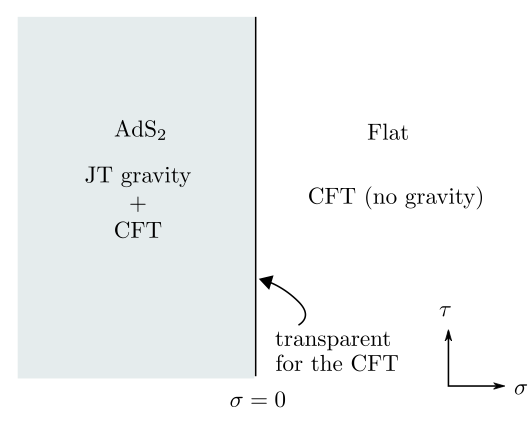
\includegraphics[scale=1]{figures/interface-setup.png}
    \end{center}
    \caption{We consider nearly-$AdS_2$ gravity with a matter CFT. The same CFT lives in an exterior flat space with no gravity. We have transparent boundary conditions for the CFT.  }
    \label{AdSandFlat}
\end{figure}



In this section we specify in more detail the theory under consideration. We have the 
Jackiw-Teitelboim gravity theory describing a nearly $AdS_2$ spacetime coupled to a matter theory that is
a CFT. In addition, we have the same  CFT  living in an  exterior flat and rigid geometry with no gravity. Since the interior and the exterior involve the same   CFT we can impose  transparent boundary conditions at the boundary,
see figure \ref{AdSandFlat}. In other words,  we have the action 
\be \la{OrigAct}
 \log Z^{\rm tot} =   { S_0 \over 4 \pi }  \left[ \int_{\Sigma_2} R +   \int_{\partial \Sigma_2} 2 K \right] + \int_{\Sigma_2} { \phi \over 4 \pi} (R+2) + { \phi_b \over 4 \pi}  \int_{\partial \Sigma_2} 2 K    + \log Z_{CFT}[g]
 \ee
 where the CFT action is defined over a geometry which is rigid in the exterior region and is dynamical in the interior region.   
 We are setting $4G_N=1$ so that the area terms in the entropies will be just given by the value of $\phi$, ${{\rm Area } \over 4 G_N} = S_0 + \phi$. 
 
 In this theory,  we want to consider the replica manifolds described above, see figure \ref{fig:manyreplicas}. Because we consider replica symmetric solutions, it is convenient to quotient by $Z_n$ and discuss a single manifold with $n$ copies of the matter theory on it. 
 In other words, we go from the action \nref{OrigAct} on $\widetilde {\cal M}_n$ to a problem 
 on ${\cal M}_n = \widetilde {\cal M}_n/Z_n $. We find that this simplifies a bit the description of the manifold, see figure \ref{CoverThree}. Namely, the manifold ${\cal M}_n$  can be viewed as a disk with conical singularities and with twist operators for the matter theory inserted at these singularities. These are the cosmic branes discussed in section \ref{sec:CosmicStrings}. The final gravitational action is as in  \nref{OrigAct} but 
  with an additional factor of $n$ and extra terms that produce the conical singularities 
  \be \la{newgra}
  -{ 1 \over n} I_{\rm grav} =  
{  S_0 \over 4 \pi }  \left[ \int_{\Sigma_2} R +   \int_{\partial \Sigma_2} 2 K \right] +  \int_{\Sigma_2} { \phi \over 4 \pi} (R+2) +  { \phi_b \over 4 \pi}  \int_{\partial \Sigma_2} 2 K  -  (1-{1 \over n}) \sum_i [ S_0 + \phi(w_i) ]
\ee
where $w_i$ are the positions of the conical singularities, or cosmic branes (which are just instantons  or -1 branes). 
We can consider \nref{newgra} as a new gravity theory and add $n$ copies of the CFT. In addition, 
we put twist fields at the positions $w_i$ of the cosmic branes.  It might look like we are breaking reparametrization invariance when when add these terms.  Reparametrization symmetry is restored because $w_i$ are dynamical variables which can be anywhere on the manifold and will be fixed by the equations of motion. 


 We treat the CFT as a quantum theory and evaluate its partition function. Then we solve the classical equations for the metric and dilaton inserting the quantum expectation value of the stress tensor. This approximation is particularly appropriate when the central charge is large $c\gg 1$. 
 So we imagine that we are in that regime for the simple euclidean solutions we discuss here. The approximation can also be justified in other regimes where  the entanglement entropy of matter is large for kinematical reasons.  
 However, this description is {\it not} correct when we need to include the quantum aspects of gravity. That computation should be done in the original manifold and the fact that the fluctuations can break the replica symmetry is important. 
 
  \begin{figure}[t]
    \begin{center}
    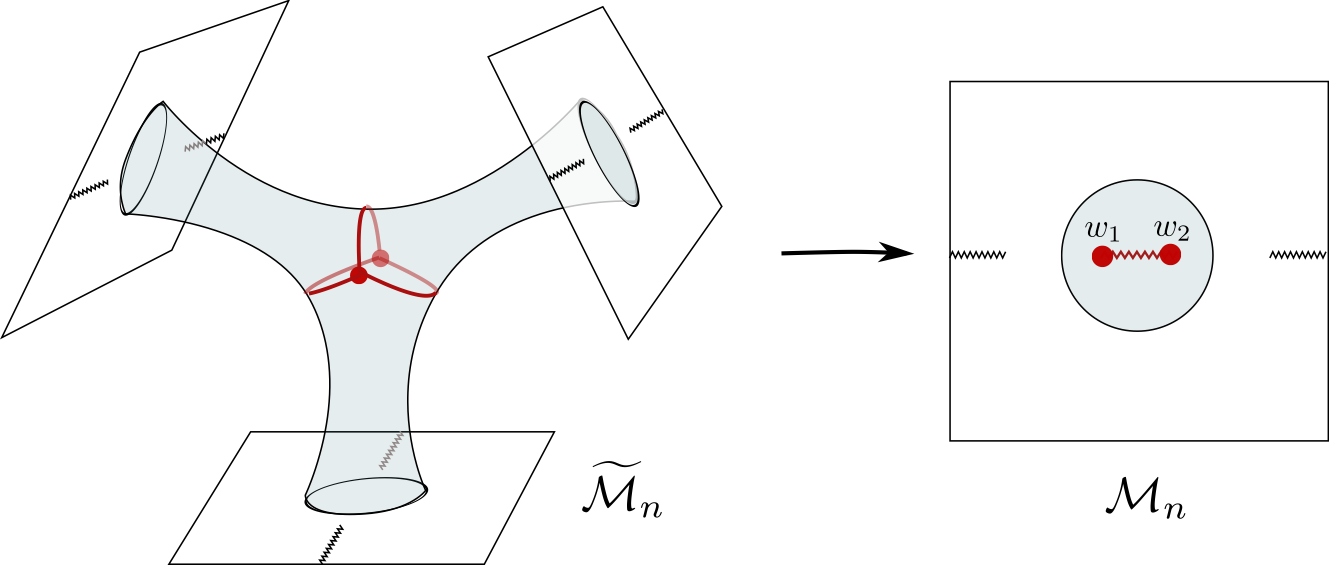
\includegraphics[scale=0.65]{figures/threereplicas.png}
    \end{center}
    \caption{Here we display the replica manifold, $\widetilde {\cal M}_3$, 
    and also the manifold ${\cal M}_3 = \widetilde {\cal M}_3/Z_3$ which has the topology of the disk with conical singularities at two points $w_1$ and $w_2$ which corresponds to the fixed points of the $Z_3$ action on $\widetilde {\cal M}_3$. We parametrize this disk in terms of the holomorphic coordinate $w$. The exterior regions of $\widetilde{\cal M}_n$ are also glued together cyclically along the cuts. }
    \label{CoverThree}
\end{figure}

 
    
 We can define an interior 
  complex coordinate $w$ where the metric for the manifold ${\cal M}_n$ in the gravitational region is  
  \be
   ds^2 = e^{ 2 \rho } d w d \bar w   ~,~~~~~{\rm with} ~~ |w| \leq 1\,. \la{MetrDis}
   \ee
   The boundary of $AdS_2$ is at $|w|=1$, or $w = e^{ i \theta} $.   
   \eqref{MetrDis} is a constant curvature metric on the disk $|w|\leq 1$ with conical singularities
   at certain values $w_i$ with opening angle $2\pi/n$. This type of metric is enforced by the dilaton equation of motion in \nref{newgra} 
  \be \la{RhoEq}
 - 4 \partial_w \partial_{\bar w} \rho +
    e^{  2 \rho} = 2 \pi (1 - { 1 \over n } ) \sum_i \delta^2(w -w_i) 
   \ee
   On this space we have $n$ copies of 
   the CFT and we have twist fields inserted at the conical singularities. 
   Notice that once we impose this equation,  the contributions in    \nref{newgra}  from the delta functions in the curvature cancel against the explicit cosmic brane action terms, as we anticipated in section \ref{sec:CosmicStrings}.    
   
   
   This metric should be joined to the flat space outside.
    We consider a finite temperature 
   configuration where $\tau \sim \tau + 2 \pi$. For general temperatures,  all we need to do is to rescale $\phi_r \to  2 \pi \phi_r/\beta $. In other words,
    the only dimensionful scale is $\phi_r$, so the only dependence on the temperature for dimensionless quantities   is through $\phi_r/\beta$.   
   We   define the coordinate $v = e^y$. So the physical half cylinder $\sigma \geq 0$ corresponds to $|v|\geq 1$. 
   At the boundary we have that $w = e^{ i \theta(\tau)}$, $v = e^{ i \tau }$. 
   Unfortunately,  we cannot extend this to a holomorphic map in the interior of the disk.
    However, we can find another coordinate $z$ such that there are holomorphic maps from $|w|\leq 1$ and $|v|\geq 1$ to the coordinate $z$, see figure \ref{WandZplanes}. 
   
   \begin{figure}[t]
    \begin{center}
    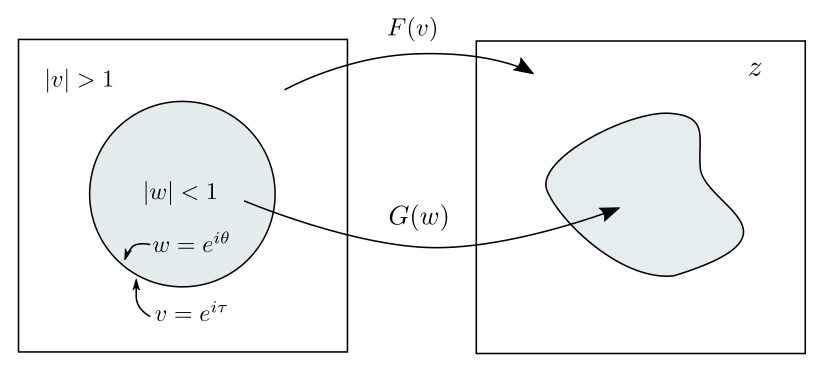
\includegraphics[scale=1]{figures/welding.png}
    \end{center}
    \caption{ The conformal welding problem.  We are given two disks, one parametrized by
     $|w|\leq 1$ and another by
    $|v| \geq 1$ with their boundaries glued in terms of a given function $\theta(\tau)$ where
    $w =e^{i\theta}$ and $v=e^{i\tau}$. Then we need to find holomorphic maps of each disk to a region of the complex $z$ plane so that they are compatible at the boundary. The functions $F$ and $G$ are only required to be holomorphic inside their respective disks.   }
    \label{WandZplanes}
\end{figure}
   
   In other words, it is possible to find two functions $G$ and $F $ such that 
   \bea \la{WeldEqns}
    z &=& G(w) ~,~~~{\rm for}~~~|w|\leq 1 ~
    \cr  ~~~~~~ z &=& F(v) ~,~~~~{\rm for}~~~|v|\geq  1 
   \cr
   &~&  G(e^{ i\theta(\tau)}) = F(e^{i\tau} ) ~,~~~{\rm for} ~~~|w|=|v|=1\,.
   \eea
   The functions $F$ and $G$ are holomorphic in their respective domains (they do not have to be holomorphic at the boundary). 
   The problem of finding $F$ and $G$ given $\theta(\tau)$ is called the 
   ``conformal welding problem,'' see \cite{Mumford} for a nice discussion.\footnote{We thank 
   L. Iliesiu and Z. Yang for discussions on this problem, and A. Lupsasca for pointing out the connection to \cite{Mumford}.}  $F$ and $G$   end up depending non-locally on $\theta(\tau)$ and they
     map the inside and outside disks to the inside and outside of some irregular region in the complex plane, see figure \ref{WandZplanes}. In our problem, $\theta(\tau)$ arises as the reparametrization mode, or ``boundary 
     graviton'' of the nearly-$AdS_2$ gravity theory \cite{Jensen:2016pah,Maldacena:2016upp,Engelsoy:2016xyb}.
   
   When $n=1$, we have a trivial stress tensor in the $z$ plane. We then insert the twist operators in the outside region, and also in the inside region. We are free to insert as many
    conical singularities and twist fields in the inside as we want. This amounts to considering various numbers of islands in the gravity region. We will only discuss cases with one or two inside insertions in the subsequent sections. 
     This gives us a non-trivial stress tensor $T_{zz}(z)$ and $T_{\bar z \bar z}(\bar z)$. We can then compute the physical stress tensor that will appear in the equation of motion using the 
   conformal anomaly, 
   \be \la{StressT}
    T_{yy} = \left( { d F(e^{ i y} ) \over dy } \right)^2 T_{zz} - 
    { c \over 24 \pi } \{ F(e^{i y}), y \} 
    \ee
    and a similar expression for $T_{\bar y \bar y } $. The expression for the physical stress tensor in the $w$ plane  involves the function $G$ and also a conformal anomaly contribution from $\rho$ in the metric \nref{MetrDis}.
    
  Let us now turn to the problem of writing the equations of motion for the boundary reparametrization mode.  
  Naively we are tempted to write the action just as    $\{ e^{ i\theta } , \tau \}$. This would be correct if there were no conical singularities in the interior. However, the presence of those conical singularities implies that the metric \nref{MetrDis} has small deviations
    compared to the metric of a standard hyperbolic disk 
    \be \la{Metdr}
    ds^2 = e^{ 2 \rho} dw d\bar w ~,~~~~~~~ e^{ 2 \rho} = { 4 \over (1 - |w|^2)^2 } e^{ 2 \delta \rho } 
    \ee
    where $\delta \rho $ goes as 
    \be \la{DelRhoe}
     \delta \rho  \sim -{ (1-|w|)^2 \over 3 } U(\theta)  ~,~~~~~{\rm as}~~~|w| \to 1\,.
     \ee 
   The function $U$ depends on the positions of the conical singularities and therefore also on
   the moduli of the Riemann surface. 
   This then implies that the Schwarzian term, and the full equation of motion can now be written as 
   \be \la{EOMFin}
   { \phi_r \over 2 \pi } { d \over d \tau } \left[ \{ e^{ i \theta} , \tau \} + U(\theta) {\theta'}^2  \right] = i (T_{yy} - T_{\bar y \bar y } ) = T_{\tau \sigma}\,.
   \ee
   The term in brackets is proportional to the energy.  This equation relates the change in energy  to the energy flux from the flat space region. Here the flux of energy on the right hand side is that of one copy, or the flux of the $n$ copies divided by $n$. 
   The action can be derived from the extrinsic curvature term in the same way that was discussed in 
  \cite{Jensen:2016pah,Maldacena:2016upp,Engelsoy:2016xyb}, see appendix \ref{GravAct}, where we also discuss the 
  explicit derivation of the equation of motion \nref{EOMFin}. 
   
   There are also equations that result from varying the moduli of the Riemann surface, or the 
   positions of the conical singularities. They  have the form 
   \be \la{PartSing}
    -(1 - { 1 \over n}) \partial_{w} \phi(w_i) + \partial_{w_i } \left( { \log Z^{\rm mat}_n \over n } \right) =0 \,,
   \ee 
   where we used that the $w_i$ dependence of the gravitational part of the action comes only from the last term in \nref{newgra}.   
  
  In the $n\to 1$ limit we can replace the $n=1$ value for the dilaton in 
   \nref{PartSing}. Similarly the value of $\log Z^{\rm mat}_n/n$ near $n=1$ involves the matter entropy. 
   Therefore \nref{PartSing}  reduces to the condition on the extremization of the generalized 
   entropy, as we discussed in general above. 
   
   For general $n$, we need to compute the dilaton by solving its equations of motion 
   in order to write  \nref{PartSing}. This can be done using the expression for the stress tensor in the interior of the disk.   
    We have not attempted to simplify it further. However, we should note that for the particular case of one interval, discussed in section \ref{sec:SingleInterval}, there is only one point and there are no moduli for the Riemann surface. Therefore this equation is redundant and in fact, it is contained in \nref{EOMFin} as will be discussed in section \ref{sec:SingleInterval}. 
  
 Next we apply this general discussion to the calculation of the entropy of various subregions of the flat space CFT. The goal is to understand how configurations of the gravity region contribute to the entropy of those CFT regions.
